% Options for packages loaded elsewhere
\PassOptionsToPackage{unicode}{hyperref}
\PassOptionsToPackage{hyphens}{url}
%
\documentclass[
]{article}
\usepackage{amsmath,amssymb}
\usepackage{lmodern}
\usepackage{iftex}
\ifPDFTeX
  \usepackage[T1]{fontenc}
  \usepackage[utf8]{inputenc}
  \usepackage{textcomp} % provide euro and other symbols
\else % if luatex or xetex
  \usepackage{unicode-math}
  \defaultfontfeatures{Scale=MatchLowercase}
  \defaultfontfeatures[\rmfamily]{Ligatures=TeX,Scale=1}
\fi
% Use upquote if available, for straight quotes in verbatim environments
\IfFileExists{upquote.sty}{\usepackage{upquote}}{}
\IfFileExists{microtype.sty}{% use microtype if available
  \usepackage[]{microtype}
  \UseMicrotypeSet[protrusion]{basicmath} % disable protrusion for tt fonts
}{}
\makeatletter
\@ifundefined{KOMAClassName}{% if non-KOMA class
  \IfFileExists{parskip.sty}{%
    \usepackage{parskip}
  }{% else
    \setlength{\parindent}{0pt}
    \setlength{\parskip}{6pt plus 2pt minus 1pt}}
}{% if KOMA class
  \KOMAoptions{parskip=half}}
\makeatother
\usepackage{xcolor}
\usepackage[margin=1in]{geometry}
\usepackage{color}
\usepackage{fancyvrb}
\newcommand{\VerbBar}{|}
\newcommand{\VERB}{\Verb[commandchars=\\\{\}]}
\DefineVerbatimEnvironment{Highlighting}{Verbatim}{commandchars=\\\{\}}
% Add ',fontsize=\small' for more characters per line
\usepackage{framed}
\definecolor{shadecolor}{RGB}{248,248,248}
\newenvironment{Shaded}{\begin{snugshade}}{\end{snugshade}}
\newcommand{\AlertTok}[1]{\textcolor[rgb]{0.94,0.16,0.16}{#1}}
\newcommand{\AnnotationTok}[1]{\textcolor[rgb]{0.56,0.35,0.01}{\textbf{\textit{#1}}}}
\newcommand{\AttributeTok}[1]{\textcolor[rgb]{0.77,0.63,0.00}{#1}}
\newcommand{\BaseNTok}[1]{\textcolor[rgb]{0.00,0.00,0.81}{#1}}
\newcommand{\BuiltInTok}[1]{#1}
\newcommand{\CharTok}[1]{\textcolor[rgb]{0.31,0.60,0.02}{#1}}
\newcommand{\CommentTok}[1]{\textcolor[rgb]{0.56,0.35,0.01}{\textit{#1}}}
\newcommand{\CommentVarTok}[1]{\textcolor[rgb]{0.56,0.35,0.01}{\textbf{\textit{#1}}}}
\newcommand{\ConstantTok}[1]{\textcolor[rgb]{0.00,0.00,0.00}{#1}}
\newcommand{\ControlFlowTok}[1]{\textcolor[rgb]{0.13,0.29,0.53}{\textbf{#1}}}
\newcommand{\DataTypeTok}[1]{\textcolor[rgb]{0.13,0.29,0.53}{#1}}
\newcommand{\DecValTok}[1]{\textcolor[rgb]{0.00,0.00,0.81}{#1}}
\newcommand{\DocumentationTok}[1]{\textcolor[rgb]{0.56,0.35,0.01}{\textbf{\textit{#1}}}}
\newcommand{\ErrorTok}[1]{\textcolor[rgb]{0.64,0.00,0.00}{\textbf{#1}}}
\newcommand{\ExtensionTok}[1]{#1}
\newcommand{\FloatTok}[1]{\textcolor[rgb]{0.00,0.00,0.81}{#1}}
\newcommand{\FunctionTok}[1]{\textcolor[rgb]{0.00,0.00,0.00}{#1}}
\newcommand{\ImportTok}[1]{#1}
\newcommand{\InformationTok}[1]{\textcolor[rgb]{0.56,0.35,0.01}{\textbf{\textit{#1}}}}
\newcommand{\KeywordTok}[1]{\textcolor[rgb]{0.13,0.29,0.53}{\textbf{#1}}}
\newcommand{\NormalTok}[1]{#1}
\newcommand{\OperatorTok}[1]{\textcolor[rgb]{0.81,0.36,0.00}{\textbf{#1}}}
\newcommand{\OtherTok}[1]{\textcolor[rgb]{0.56,0.35,0.01}{#1}}
\newcommand{\PreprocessorTok}[1]{\textcolor[rgb]{0.56,0.35,0.01}{\textit{#1}}}
\newcommand{\RegionMarkerTok}[1]{#1}
\newcommand{\SpecialCharTok}[1]{\textcolor[rgb]{0.00,0.00,0.00}{#1}}
\newcommand{\SpecialStringTok}[1]{\textcolor[rgb]{0.31,0.60,0.02}{#1}}
\newcommand{\StringTok}[1]{\textcolor[rgb]{0.31,0.60,0.02}{#1}}
\newcommand{\VariableTok}[1]{\textcolor[rgb]{0.00,0.00,0.00}{#1}}
\newcommand{\VerbatimStringTok}[1]{\textcolor[rgb]{0.31,0.60,0.02}{#1}}
\newcommand{\WarningTok}[1]{\textcolor[rgb]{0.56,0.35,0.01}{\textbf{\textit{#1}}}}
\usepackage{graphicx}
\makeatletter
\def\maxwidth{\ifdim\Gin@nat@width>\linewidth\linewidth\else\Gin@nat@width\fi}
\def\maxheight{\ifdim\Gin@nat@height>\textheight\textheight\else\Gin@nat@height\fi}
\makeatother
% Scale images if necessary, so that they will not overflow the page
% margins by default, and it is still possible to overwrite the defaults
% using explicit options in \includegraphics[width, height, ...]{}
\setkeys{Gin}{width=\maxwidth,height=\maxheight,keepaspectratio}
% Set default figure placement to htbp
\makeatletter
\def\fps@figure{htbp}
\makeatother
\setlength{\emergencystretch}{3em} % prevent overfull lines
\providecommand{\tightlist}{%
  \setlength{\itemsep}{0pt}\setlength{\parskip}{0pt}}
\setcounter{secnumdepth}{-\maxdimen} % remove section numbering
\ifLuaTeX
  \usepackage{selnolig}  % disable illegal ligatures
\fi
\IfFileExists{bookmark.sty}{\usepackage{bookmark}}{\usepackage{hyperref}}
\IfFileExists{xurl.sty}{\usepackage{xurl}}{} % add URL line breaks if available
\urlstyle{same} % disable monospaced font for URLs
\hypersetup{
  pdftitle={PSTAT 131 Homework 6},
  pdfauthor={Sunrise Gao},
  hidelinks,
  pdfcreator={LaTeX via pandoc}}

\title{PSTAT 131 Homework 6}
\author{Sunrise Gao}
\date{11/20/2022}

\begin{document}
\maketitle

{
\setcounter{tocdepth}{2}
\tableofcontents
}
\hypertarget{tree-based-models}{%
\subsection{Tree-Based Models}\label{tree-based-models}}

For this assignment, we will continue working with the file
\texttt{"pokemon.csv"}, found in \texttt{/data}. The file is from
Kaggle: \url{https://www.kaggle.com/abcsds/pokemon}.

The \href{https://www.pokemon.com/us/}{Pokémon} franchise encompasses
video games, TV shows, movies, books, and a card game. This data set was
drawn from the video game series and contains statistics about 721
Pokémon, or ``pocket monsters.'' In Pokémon games, the user plays as a
trainer who collects, trades, and battles Pokémon to (a) collect all the
Pokémon and (b) become the champion Pokémon trainer.

Each Pokémon has a
\href{https://bulbapedia.bulbagarden.net/wiki/Type}{primary type} (some
even have secondary types). Based on their type, a Pokémon is strong
against some types, and vulnerable to others. (Think rock, paper,
scissors.) A Fire-type Pokémon, for example, is vulnerable to Water-type
Pokémon, but strong against Grass-type.

\begin{figure}
\centering
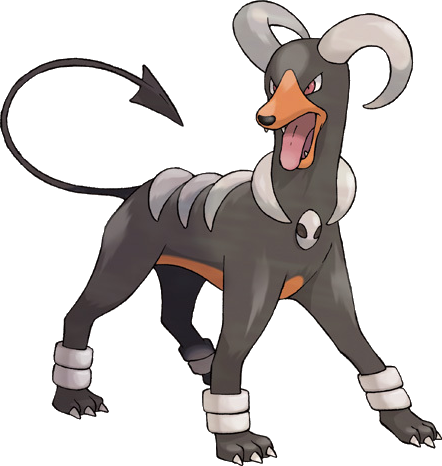
\includegraphics[width=2.08333in,height=\textheight]{images/houndoom.jpg}
\caption{Fig 1. Houndoom, a Dark/Fire-type canine Pokémon from
Generation II.}
\end{figure}

The goal of this assignment is to build a statistical learning model
that can predict the \textbf{primary type} of a Pokémon based on its
generation, legendary status, and six battle statistics.

\textbf{Note: Fitting ensemble tree-based models can take a little while
to run. Consider running your models outside of the .Rmd, storing the
results, and loading them in your .Rmd to minimize time to knit.}

\begin{Shaded}
\begin{Highlighting}[]
\FunctionTok{library}\NormalTok{(tidymodels)}
\FunctionTok{library}\NormalTok{(tidyverse)}

\FunctionTok{library}\NormalTok{(ISLR) }\CommentTok{\# For the Smarket data set}
\FunctionTok{library}\NormalTok{(ISLR2) }\CommentTok{\# For the Bikeshare data set}
\FunctionTok{library}\NormalTok{(klaR) }\CommentTok{\# for naive bayes}

\FunctionTok{library}\NormalTok{(discrim)}
\FunctionTok{library}\NormalTok{(poissonreg)}
\FunctionTok{library}\NormalTok{(corrr)}
\FunctionTok{library}\NormalTok{(forcats)}
\FunctionTok{library}\NormalTok{(corrplot)}
\FunctionTok{library}\NormalTok{(pROC)}
\FunctionTok{library}\NormalTok{(recipes)}
\FunctionTok{library}\NormalTok{(rsample)}
\FunctionTok{library}\NormalTok{(parsnip)}
\FunctionTok{library}\NormalTok{(workflows)}
\FunctionTok{library}\NormalTok{(janitor)}
\FunctionTok{library}\NormalTok{(glmnet)}
\FunctionTok{library}\NormalTok{(rpart.plot)}
\FunctionTok{library}\NormalTok{(vip)}
\FunctionTok{library}\NormalTok{(janitor)}
\FunctionTok{library}\NormalTok{(randomForest)}
\FunctionTok{library}\NormalTok{(xgboost)}
\FunctionTok{tidymodels\_prefer}\NormalTok{()}
\end{Highlighting}
\end{Shaded}

\hypertarget{exercise-1}{%
\subsubsection{Exercise 1}\label{exercise-1}}

Read in the data and set things up as in Homework 5:

\begin{itemize}
\tightlist
\item
  Use \texttt{clean\_names()}
\item
  Filter out the rarer Pokémon types
\item
  Convert \texttt{type\_1} and \texttt{legendary} to factors
\end{itemize}

Do an initial split of the data; you can choose the percentage for
splitting. Stratify on the outcome variable.

Fold the training set using \emph{v}-fold cross-validation, with
\texttt{v\ =\ 5}. Stratify on the outcome variable.

Set up a recipe to predict \texttt{type\_1} with \texttt{legendary},
\texttt{generation}, \texttt{sp\_atk}, \texttt{attack}, \texttt{speed},
\texttt{defense}, \texttt{hp}, and \texttt{sp\_def}:

\begin{itemize}
\tightlist
\item
  Dummy-code \texttt{legendary} and \texttt{generation};
\item
  Center and scale all predictors.
\end{itemize}

\begin{Shaded}
\begin{Highlighting}[]
\CommentTok{\# read dataset}
\NormalTok{pokemon\_raw }\OtherTok{\textless{}{-}} \FunctionTok{read.csv}\NormalTok{(}\StringTok{"Pokemon.csv"}\NormalTok{) }

\CommentTok{\# clean\_name()}
\NormalTok{pokemon1 }\OtherTok{\textless{}{-}} \FunctionTok{clean\_names}\NormalTok{(pokemon\_raw)}

\CommentTok{\# filter out rarer}
\NormalTok{pokemon }\OtherTok{\textless{}{-}}\NormalTok{ pokemon1[}\FunctionTok{which}\NormalTok{(pokemon1}\SpecialCharTok{$}\NormalTok{type\_1 }\SpecialCharTok{==} \StringTok{"Bug"}\SpecialCharTok{|}\NormalTok{ pokemon1}\SpecialCharTok{$}\NormalTok{type\_1 }\SpecialCharTok{==}\StringTok{"Fire"}\SpecialCharTok{|}
\NormalTok{                     pokemon1}\SpecialCharTok{$}\NormalTok{type\_1 }\SpecialCharTok{==}\StringTok{"Grass"}\SpecialCharTok{|}\NormalTok{ pokemon1}\SpecialCharTok{$}\NormalTok{type\_1 }\SpecialCharTok{==}\StringTok{"Normal"}\SpecialCharTok{|} 
\NormalTok{                     pokemon1}\SpecialCharTok{$}\NormalTok{type\_1 }\SpecialCharTok{==}\StringTok{"Water"}\SpecialCharTok{|}\NormalTok{ pokemon1}\SpecialCharTok{$}\NormalTok{type\_1 }\SpecialCharTok{==}\StringTok{"Psychic"}\NormalTok{), ]}

\CommentTok{\# convert factors}
\NormalTok{pokemon }\OtherTok{\textless{}{-}}\NormalTok{ pokemon }\SpecialCharTok{\%\textgreater{}\%} 
              \FunctionTok{mutate}\NormalTok{(}\AttributeTok{type\_1 =} \FunctionTok{factor}\NormalTok{(type\_1), }
                  \AttributeTok{legendary =}\FunctionTok{factor}\NormalTok{(legendary))}

\CommentTok{\# initial split}
\FunctionTok{set.seed}\NormalTok{(}\DecValTok{2022}\NormalTok{)}
\NormalTok{pokemon\_split }\OtherTok{\textless{}{-}}\NormalTok{ pokemon }\SpecialCharTok{\%\textgreater{}\%} 
  \FunctionTok{initial\_split}\NormalTok{(}\AttributeTok{strata =}\NormalTok{ type\_1, }\AttributeTok{prop =} \FloatTok{0.7}\NormalTok{)}
\NormalTok{pokemon\_train }\OtherTok{\textless{}{-}} \FunctionTok{training}\NormalTok{(pokemon\_split)}
\NormalTok{pokemon\_test }\OtherTok{\textless{}{-}} \FunctionTok{testing}\NormalTok{(pokemon\_split)}

\CommentTok{\# set up cross{-}validation}
\NormalTok{pokemon\_fold }\OtherTok{\textless{}{-}} \FunctionTok{vfold\_cv}\NormalTok{(pokemon\_train, }\AttributeTok{v =} \DecValTok{5}\NormalTok{, }\AttributeTok{strata =}\NormalTok{ type\_1)}

\CommentTok{\# set up recipe}
\NormalTok{pokemon\_recipe }\OtherTok{\textless{}{-}} \FunctionTok{recipe}\NormalTok{(type\_1 }\SpecialCharTok{\textasciitilde{}}\NormalTok{ legendary }\SpecialCharTok{+}\NormalTok{ generation }\SpecialCharTok{+}\NormalTok{ sp\_atk }\SpecialCharTok{+} 
\NormalTok{                         attack }\SpecialCharTok{+}\NormalTok{ speed }\SpecialCharTok{+}\NormalTok{ defense }\SpecialCharTok{+}\NormalTok{ hp }\SpecialCharTok{+}\NormalTok{ sp\_def, pokemon\_train) }\SpecialCharTok{\%\textgreater{}\%} 
  \FunctionTok{step\_dummy}\NormalTok{(legendary,generation) }\SpecialCharTok{\%\textgreater{}\%} 
  \FunctionTok{step\_center}\NormalTok{(}\FunctionTok{all\_predictors}\NormalTok{()) }\SpecialCharTok{\%\textgreater{}\%}
  \FunctionTok{step\_scale}\NormalTok{(}\FunctionTok{all\_predictors}\NormalTok{())}
\end{Highlighting}
\end{Shaded}

\hypertarget{exercise-2}{%
\subsubsection{Exercise 2}\label{exercise-2}}

Create a correlation matrix of the training set, using the
\texttt{corrplot} package. \emph{Note: You can choose how to handle the
continuous variables for this plot; justify your decision(s).}

What relationships, if any, do you notice? Do these relationships make
sense to you?

\begin{Shaded}
\begin{Highlighting}[]
\NormalTok{pokemon\_train }\SpecialCharTok{\%\textgreater{}\%} 
  \FunctionTok{select}\NormalTok{(}\FunctionTok{where}\NormalTok{(is.numeric), }\SpecialCharTok{{-}}\NormalTok{x,}\SpecialCharTok{{-}}\NormalTok{generation) }\SpecialCharTok{\%\textgreater{}\%} 
  \FunctionTok{cor}\NormalTok{(}\AttributeTok{use =} \StringTok{"complete.obs"}\NormalTok{) }\SpecialCharTok{\%\textgreater{}\%} 
  \FunctionTok{corrplot}\NormalTok{(}\AttributeTok{type =} \StringTok{"lower"}\NormalTok{, }\AttributeTok{diag =} \ConstantTok{FALSE}\NormalTok{)  }
\end{Highlighting}
\end{Shaded}

\includegraphics{homework-6_files/figure-latex/unnamed-chunk-3-1.pdf}

\hfill\break
\emph{I remove variable x and generation since x is index and generation
is not continuous.}\\
\emph{Almost all the variables have positive relationship to other,
especially, all variables are high positive relate to total which make
sense to me that the higher variable a pokemon has the more stronger
pokemon is.}

\hypertarget{exercise-3}{%
\subsubsection{Exercise 3}\label{exercise-3}}

First, set up a decision tree model and workflow. Tune the
\texttt{cost\_complexity} hyperparameter. Use the same levels we used in
Lab 7 -- that is, \texttt{range\ =\ c(-3,\ -1)}. Specify that the metric
we want to optimize is \texttt{roc\_auc}.

Print an \texttt{autoplot()} of the results. What do you observe? Does a
single decision tree perform better with a smaller or larger complexity
penalty?

\begin{Shaded}
\begin{Highlighting}[]
\CommentTok{\# set up model and workflow}
\NormalTok{tree\_spec }\OtherTok{\textless{}{-}} \FunctionTok{decision\_tree}\NormalTok{() }\SpecialCharTok{\%\textgreater{}\%}
  \FunctionTok{set\_engine}\NormalTok{(}\StringTok{"rpart"}\NormalTok{)}

\NormalTok{class\_tree\_spec }\OtherTok{\textless{}{-}}\NormalTok{ tree\_spec }\SpecialCharTok{\%\textgreater{}\%}
  \FunctionTok{set\_mode}\NormalTok{(}\StringTok{"classification"}\NormalTok{)}

\NormalTok{class\_tree\_wf }\OtherTok{\textless{}{-}} \FunctionTok{workflow}\NormalTok{() }\SpecialCharTok{\%\textgreater{}\%}
  \FunctionTok{add\_recipe}\NormalTok{(pokemon\_recipe) }\SpecialCharTok{\%\textgreater{}\%}
  \FunctionTok{add\_model}\NormalTok{(class\_tree\_spec }\SpecialCharTok{\%\textgreater{}\%} 
  \FunctionTok{set\_args}\NormalTok{(}\AttributeTok{cost\_complexity =} \FunctionTok{tune}\NormalTok{())) }
 

\NormalTok{param\_grid }\OtherTok{\textless{}{-}} \FunctionTok{grid\_regular}\NormalTok{(}\FunctionTok{cost\_complexity}\NormalTok{(}\AttributeTok{range =} \FunctionTok{c}\NormalTok{(}\SpecialCharTok{{-}}\DecValTok{3}\NormalTok{, }\SpecialCharTok{{-}}\DecValTok{1}\NormalTok{)), }\AttributeTok{levels =} \DecValTok{10}\NormalTok{)}

\NormalTok{tune\_res }\OtherTok{\textless{}{-}} \FunctionTok{tune\_grid}\NormalTok{(}
\NormalTok{  class\_tree\_wf, }
  \AttributeTok{resamples =}\NormalTok{ pokemon\_fold, }
  \AttributeTok{grid =}\NormalTok{ param\_grid, }
  \AttributeTok{metrics =} \FunctionTok{metric\_set}\NormalTok{(roc\_auc)}
\NormalTok{)}

\CommentTok{\# print results}
\FunctionTok{autoplot}\NormalTok{(tune\_res)}
\end{Highlighting}
\end{Shaded}

\includegraphics{homework-6_files/figure-latex/unnamed-chunk-4-1.pdf}

\hfill\break
\emph{The roc\_auc stays around 0.615 and doesn't change a lot with the
increasing of parameter, and reaches the peak around 0.02 of the
parameter value. After that, the roc\_auc starts dropping rapidly after
around 0.075 of the parameter value.}\\
\emph{So, we can see that a single decision tree perform better with a
larger complexity penalty.}

\hypertarget{exercise-4}{%
\subsubsection{Exercise 4}\label{exercise-4}}

What is the \texttt{roc\_auc} of your best-performing pruned decision
tree on the folds? \emph{Hint: Use \texttt{collect\_metrics()} and
\texttt{arrange()}.}

\begin{Shaded}
\begin{Highlighting}[]
\FunctionTok{arrange}\NormalTok{(}\FunctionTok{collect\_metrics}\NormalTok{(tune\_res),}\FunctionTok{desc}\NormalTok{(mean))}
\end{Highlighting}
\end{Shaded}

\begin{verbatim}
## # A tibble: 10 x 7
##    cost_complexity .metric .estimator  mean     n std_err .config              
##              <dbl> <chr>   <chr>      <dbl> <int>   <dbl> <chr>                
##  1         0.0215  roc_auc hand_till  0.629     5 0.0110  Preprocessor1_Model07
##  2         0.0359  roc_auc hand_till  0.629     5 0.0110  Preprocessor1_Model08
##  3         0.0599  roc_auc hand_till  0.627     5 0.0131  Preprocessor1_Model09
##  4         0.0129  roc_auc hand_till  0.624     5 0.0150  Preprocessor1_Model06
##  5         0.001   roc_auc hand_till  0.620     5 0.00860 Preprocessor1_Model01
##  6         0.00167 roc_auc hand_till  0.620     5 0.00860 Preprocessor1_Model02
##  7         0.00278 roc_auc hand_till  0.620     5 0.00860 Preprocessor1_Model03
##  8         0.00464 roc_auc hand_till  0.620     5 0.00860 Preprocessor1_Model04
##  9         0.00774 roc_auc hand_till  0.616     5 0.0139  Preprocessor1_Model05
## 10         0.1     roc_auc hand_till  0.526     5 0.0262  Preprocessor1_Model10
\end{verbatim}

\hfill\break
\emph{0.629 roc\_auc along with 0.0215 parameter is the best model.}

\hypertarget{exercise-5}{%
\subsubsection{Exercise 5}\label{exercise-5}}

Using \texttt{rpart.plot}, fit and visualize your best-performing pruned
decision tree with the \emph{training} set.

\begin{Shaded}
\begin{Highlighting}[]
\NormalTok{best\_complexity }\OtherTok{\textless{}{-}} \FunctionTok{select\_best}\NormalTok{(tune\_res)}

\NormalTok{class\_tree\_final }\OtherTok{\textless{}{-}} \FunctionTok{finalize\_workflow}\NormalTok{(class\_tree\_wf, best\_complexity)}

\NormalTok{class\_tree\_final\_fit }\OtherTok{\textless{}{-}} \FunctionTok{fit}\NormalTok{(class\_tree\_final, }\AttributeTok{data =}\NormalTok{ pokemon\_train)}

\NormalTok{class\_tree\_final\_fit }\SpecialCharTok{\%\textgreater{}\%}
  \FunctionTok{extract\_fit\_engine}\NormalTok{() }\SpecialCharTok{\%\textgreater{}\%}
  \FunctionTok{rpart.plot}\NormalTok{()}
\end{Highlighting}
\end{Shaded}

\includegraphics{homework-6_files/figure-latex/unnamed-chunk-6-1.pdf}

\hypertarget{exercise-5-1}{%
\subsubsection{Exercise 5}\label{exercise-5-1}}

Now set up a random forest model and workflow. Use the \texttt{ranger}
engine and set \texttt{importance\ =\ "impurity"}. Tune \texttt{mtry},
\texttt{trees}, and \texttt{min\_n}. Using the documentation for
\texttt{rand\_forest()}, explain in your own words what each of these
hyperparameters represent.

Create a regular grid with 8 levels each. You can choose plausible
ranges for each hyperparameter. Note that \texttt{mtry} should not be
smaller than 1 or larger than 8. \textbf{Explain why not. What type of
model would \texttt{mtry\ =\ 8} represent?}

\begin{Shaded}
\begin{Highlighting}[]
\NormalTok{rf\_spec }\OtherTok{\textless{}{-}} \FunctionTok{rand\_forest}\NormalTok{(}\AttributeTok{mtry =} \FunctionTok{tune}\NormalTok{(),}\AttributeTok{trees =} \FunctionTok{tune}\NormalTok{(), }\AttributeTok{min\_n =} \FunctionTok{tune}\NormalTok{()) }\SpecialCharTok{\%\textgreater{}\%}
  \FunctionTok{set\_engine}\NormalTok{(}\StringTok{"ranger"}\NormalTok{, }\AttributeTok{importance =} \StringTok{"impurity"}\NormalTok{) }\SpecialCharTok{\%\textgreater{}\%}
  \FunctionTok{set\_mode}\NormalTok{(}\StringTok{"classification"}\NormalTok{)}

\NormalTok{rf\_wf }\OtherTok{\textless{}{-}} \FunctionTok{workflow}\NormalTok{() }\SpecialCharTok{\%\textgreater{}\%}
  \FunctionTok{add\_model}\NormalTok{(rf\_spec) }\SpecialCharTok{\%\textgreater{}\%} 
  \FunctionTok{add\_recipe}\NormalTok{(pokemon\_recipe)}

\NormalTok{param\_grid2 }\OtherTok{\textless{}{-}} \FunctionTok{grid\_regular}\NormalTok{(}\FunctionTok{mtry}\NormalTok{(}\AttributeTok{range =} \FunctionTok{c}\NormalTok{(}\DecValTok{1}\NormalTok{, }\DecValTok{8}\NormalTok{)),}
                           \FunctionTok{trees}\NormalTok{(}\AttributeTok{range =} \FunctionTok{c}\NormalTok{(}\DecValTok{10}\NormalTok{, }\DecValTok{1000}\NormalTok{)),}
                           \FunctionTok{min\_n}\NormalTok{(}\AttributeTok{range =} \FunctionTok{c}\NormalTok{(}\DecValTok{1}\NormalTok{, }\DecValTok{8}\NormalTok{)),}
                           \AttributeTok{levels =} \DecValTok{8}\NormalTok{)}
\end{Highlighting}
\end{Shaded}

\begin{itemize}
\tightlist
\item
  mtry: The number of predictors will be randomly sampled with each
  split of tree models.
\item
  trees: The number of trees in the ensemble tree models.
\item
  min\_n: The minimum number of data points in a node that is required
  to make a split.
\end{itemize}

\emph{mtry should not be smaller than 1 or larger than 8 since we only
have 8 predictors.}\\
\emph{If we set mtry = 8, it will represent the bagging model.}

\hypertarget{exercise-6}{%
\subsubsection{Exercise 6}\label{exercise-6}}

Specify \texttt{roc\_auc} as a metric. Tune the model and print an
\texttt{autoplot()} of the results. What do you observe? What values of
the hyperparameters seem to yield the best performance?

\begin{Shaded}
\begin{Highlighting}[]
\NormalTok{tune\_res }\OtherTok{\textless{}{-}} \FunctionTok{tune\_grid}\NormalTok{(}
\NormalTok{  rf\_wf, }
  \AttributeTok{resamples =}\NormalTok{ pokemon\_fold, }
  \AttributeTok{grid =}\NormalTok{ param\_grid2, }
  \AttributeTok{metrics =} \FunctionTok{metric\_set}\NormalTok{(roc\_auc)}
\NormalTok{)}

\CommentTok{\# print results}
\FunctionTok{autoplot}\NormalTok{(tune\_res)}
\end{Highlighting}
\end{Shaded}

\includegraphics{homework-6_files/figure-latex/unnamed-chunk-8-1.pdf}

\hfill\break
\emph{The best model's roc\_auc is 0.747 which contains 2 mtry, 575
trees,and 4 min\_n.}\\
\emph{In general, The more trees we add the better performance we have,
and the roc\_auc and the number of predictors are negatively relative.}

\hypertarget{exercise-7}{%
\subsubsection{Exercise 7}\label{exercise-7}}

What is the \texttt{roc\_auc} of your best-performing random forest
model on the folds? \emph{Hint: Use \texttt{collect\_metrics()} and
\texttt{arrange()}.}

\begin{Shaded}
\begin{Highlighting}[]
\FunctionTok{arrange}\NormalTok{(}\FunctionTok{collect\_metrics}\NormalTok{(tune\_res),}\FunctionTok{desc}\NormalTok{(mean))}
\end{Highlighting}
\end{Shaded}

\begin{verbatim}
## # A tibble: 512 x 9
##     mtry trees min_n .metric .estimator  mean     n std_err .config             
##    <int> <int> <int> <chr>   <chr>      <dbl> <int>   <dbl> <chr>               
##  1     2   858     5 roc_auc hand_till  0.748     5  0.0128 Preprocessor1_Model~
##  2     2   575     4 roc_auc hand_till  0.747     5  0.0136 Preprocessor1_Model~
##  3     2  1000     5 roc_auc hand_till  0.747     5  0.0130 Preprocessor1_Model~
##  4     2   292     4 roc_auc hand_till  0.746     5  0.0140 Preprocessor1_Model~
##  5     2   292     7 roc_auc hand_till  0.746     5  0.0136 Preprocessor1_Model~
##  6     2  1000     6 roc_auc hand_till  0.746     5  0.0111 Preprocessor1_Model~
##  7     2   717     5 roc_auc hand_till  0.746     5  0.0126 Preprocessor1_Model~
##  8     2   717     7 roc_auc hand_till  0.746     5  0.0148 Preprocessor1_Model~
##  9     2  1000     3 roc_auc hand_till  0.745     5  0.0122 Preprocessor1_Model~
## 10     2   575     7 roc_auc hand_till  0.745     5  0.0133 Preprocessor1_Model~
## # ... with 502 more rows
\end{verbatim}

\emph{The best model's roc\_auc is 0.747 which contains 2 mtry, 575
trees,and 4 min\_n.}

\hypertarget{exercise-8}{%
\subsubsection{Exercise 8}\label{exercise-8}}

Create a variable importance plot, using \texttt{vip()}, with your
best-performing random forest model fit on the \emph{training} set.

Which variables were most useful? Which were least useful? Are these
results what you expected, or not?

\begin{Shaded}
\begin{Highlighting}[]
\NormalTok{best\_complexity }\OtherTok{\textless{}{-}} \FunctionTok{select\_best}\NormalTok{(tune\_res, }\AttributeTok{metric =} \StringTok{"roc\_auc"}\NormalTok{)}
\NormalTok{pokemon\_final }\OtherTok{\textless{}{-}} \FunctionTok{finalize\_workflow}\NormalTok{(rf\_wf, best\_complexity)}
\NormalTok{rf\_fit }\OtherTok{\textless{}{-}} \FunctionTok{fit}\NormalTok{(pokemon\_final,}\AttributeTok{data =}\NormalTok{ pokemon\_train)}
\NormalTok{rf\_fit }\SpecialCharTok{\%\textgreater{}\%}
  \FunctionTok{extract\_fit\_engine}\NormalTok{() }\SpecialCharTok{\%\textgreater{}\%}
  \FunctionTok{vip}\NormalTok{()}
\end{Highlighting}
\end{Shaded}

\includegraphics{homework-6_files/figure-latex/unnamed-chunk-10-1.pdf}

\hfill\break
\emph{The most useful variable is sp\_atk and the least useful variable
is legendary\_True, I'm so surprise that the sp\_atk is the most useful
variable, and the other variables are under my consideration.}

\hypertarget{exercise-9}{%
\subsubsection{Exercise 9}\label{exercise-9}}

Finally, set up a boosted tree model and workflow. Use the
\texttt{xgboost} engine. Tune \texttt{trees}. Create a regular grid with
10 levels; let \texttt{trees} range from 10 to 2000. Specify
\texttt{roc\_auc} and again print an \texttt{autoplot()} of the results.

What do you observe?

What is the \texttt{roc\_auc} of your best-performing boosted tree model
on the folds? \emph{Hint: Use \texttt{collect\_metrics()} and
\texttt{arrange()}.}

\begin{Shaded}
\begin{Highlighting}[]
\NormalTok{boost\_tree\_spec }\OtherTok{\textless{}{-}} \FunctionTok{boost\_tree}\NormalTok{(}\AttributeTok{trees =} \FunctionTok{tune}\NormalTok{()) }\SpecialCharTok{\%\textgreater{}\%}
  \FunctionTok{set\_engine}\NormalTok{(}\StringTok{"xgboost"}\NormalTok{) }\SpecialCharTok{\%\textgreater{}\%}
  \FunctionTok{set\_mode}\NormalTok{(}\StringTok{"classification"}\NormalTok{)}

\NormalTok{boost\_tree\_grid }\OtherTok{\textless{}{-}} \FunctionTok{grid\_regular}\NormalTok{(}\FunctionTok{trees}\NormalTok{(}\FunctionTok{c}\NormalTok{(}\DecValTok{10}\NormalTok{,}\DecValTok{2000}\NormalTok{)),}\AttributeTok{levels =} \DecValTok{10}\NormalTok{)}

\NormalTok{boost\_tree\_wf }\OtherTok{\textless{}{-}} \FunctionTok{workflow}\NormalTok{() }\SpecialCharTok{\%\textgreater{}\%}
  \FunctionTok{add\_model}\NormalTok{(boost\_tree\_spec) }\SpecialCharTok{\%\textgreater{}\%}
  \FunctionTok{add\_formula}\NormalTok{(type\_1 }\SpecialCharTok{\textasciitilde{}}\NormalTok{ sp\_atk }\SpecialCharTok{+}\NormalTok{ attack }\SpecialCharTok{+}\NormalTok{ speed }\SpecialCharTok{+} 
\NormalTok{                defense }\SpecialCharTok{+}\NormalTok{ hp }\SpecialCharTok{+}\NormalTok{ sp\_def }\SpecialCharTok{+}\NormalTok{ legendary }\SpecialCharTok{+}\NormalTok{ generation)}

\NormalTok{boost\_tune\_res }\OtherTok{\textless{}{-}} \FunctionTok{tune\_grid}\NormalTok{(}
\NormalTok{  boost\_tree\_wf, }
  \AttributeTok{resamples =}\NormalTok{ pokemon\_fold, }
  \AttributeTok{grid =}\NormalTok{ boost\_tree\_grid, }
  \AttributeTok{metrics =} \FunctionTok{metric\_set}\NormalTok{(roc\_auc),}
\NormalTok{)}
 
\FunctionTok{autoplot}\NormalTok{(boost\_tune\_res)}
\end{Highlighting}
\end{Shaded}

\includegraphics{homework-6_files/figure-latex/unnamed-chunk-11-1.pdf}

\emph{The rou\_auc keeps increasing until around 250 and starts
decreasing while the trees number is increasing.}

\begin{Shaded}
\begin{Highlighting}[]
\FunctionTok{arrange}\NormalTok{(}\FunctionTok{collect\_metrics}\NormalTok{(boost\_tune\_res),}\FunctionTok{desc}\NormalTok{(mean))}
\end{Highlighting}
\end{Shaded}

\begin{verbatim}
## # A tibble: 10 x 7
##    trees .metric .estimator  mean     n std_err .config              
##    <int> <chr>   <chr>      <dbl> <int>   <dbl> <chr>                
##  1   231 roc_auc hand_till  0.728     5  0.0179 Preprocessor1_Model02
##  2   452 roc_auc hand_till  0.726     5  0.0178 Preprocessor1_Model03
##  3   673 roc_auc hand_till  0.725     5  0.0171 Preprocessor1_Model04
##  4   894 roc_auc hand_till  0.725     5  0.0174 Preprocessor1_Model05
##  5  1336 roc_auc hand_till  0.722     5  0.0187 Preprocessor1_Model07
##  6  1557 roc_auc hand_till  0.722     5  0.0193 Preprocessor1_Model08
##  7  1115 roc_auc hand_till  0.722     5  0.0182 Preprocessor1_Model06
##  8  1778 roc_auc hand_till  0.721     5  0.0199 Preprocessor1_Model09
##  9  2000 roc_auc hand_till  0.720     5  0.0202 Preprocessor1_Model10
## 10    10 roc_auc hand_till  0.717     5  0.0167 Preprocessor1_Model01
\end{verbatim}

\emph{The best model is the one that has 0.728 roc\_auc and 231 trees.}

\hypertarget{exercise-10}{%
\subsubsection{Exercise 10}\label{exercise-10}}

Display a table of the three ROC AUC values for your best-performing
pruned tree, random forest, and boosted tree models. Which performed
best on the folds? Select the best of the three and use
\texttt{select\_best()}, \texttt{finalize\_workflow()}, and
\texttt{fit()} to fit it to the \emph{testing} set.

\begin{Shaded}
\begin{Highlighting}[]
\NormalTok{best\_boost\_tree }\OtherTok{\textless{}{-}} \FunctionTok{select\_best}\NormalTok{(boost\_tune\_res)}
\NormalTok{boost\_tree\_final }\OtherTok{\textless{}{-}} \FunctionTok{finalize\_workflow}\NormalTok{(boost\_tree\_wf, best\_boost\_tree)}
\NormalTok{boost\_tree\_final\_fit }\OtherTok{\textless{}{-}} \FunctionTok{fit}\NormalTok{(boost\_tree\_final, }\AttributeTok{data =}\NormalTok{ pokemon\_train)}
\end{Highlighting}
\end{Shaded}

\begin{Shaded}
\begin{Highlighting}[]
\NormalTok{final\_class\_model }\OtherTok{=} \FunctionTok{augment}\NormalTok{(class\_tree\_final\_fit, }\AttributeTok{new\_data =}\NormalTok{ pokemon\_train)}
\NormalTok{final\_rand\_model }\OtherTok{=} \FunctionTok{augment}\NormalTok{(rf\_fit, }\AttributeTok{new\_data =}\NormalTok{ pokemon\_train)}
\NormalTok{final\_boost\_model }\OtherTok{=} \FunctionTok{augment}\NormalTok{(boost\_tree\_final\_fit, }\AttributeTok{new\_data =}\NormalTok{ pokemon\_train)}
\NormalTok{results}\OtherTok{\textless{}{-}} \FunctionTok{bind\_rows}\NormalTok{(}
  \FunctionTok{roc\_auc}\NormalTok{(final\_class\_model, }\AttributeTok{truth =}\NormalTok{ type\_1, .pred\_Bug, .pred\_Fire, .pred\_Grass, }
\NormalTok{          .pred\_Normal, .pred\_Water, .pred\_Psychic),}
  \FunctionTok{roc\_auc}\NormalTok{(final\_rand\_model, }\AttributeTok{truth =}\NormalTok{ type\_1, .pred\_Bug, .pred\_Fire, .pred\_Grass, }
\NormalTok{          .pred\_Normal, .pred\_Water, .pred\_Psychic),}
  \FunctionTok{roc\_auc}\NormalTok{(final\_boost\_model, }\AttributeTok{truth =}\NormalTok{ type\_1, .pred\_Bug, .pred\_Fire, .pred\_Grass, }
\NormalTok{          .pred\_Normal, .pred\_Water, .pred\_Psychic) }
\NormalTok{)}
\NormalTok{results}
\end{Highlighting}
\end{Shaded}

\begin{verbatim}
## # A tibble: 3 x 3
##   .metric .estimator .estimate
##   <chr>   <chr>          <dbl>
## 1 roc_auc hand_till      0.598
## 2 roc_auc hand_till      0.796
## 3 roc_auc hand_till      0.795
\end{verbatim}

\emph{We see that the best model is random forest which has roc\_auc is
0.796.}

\begin{Shaded}
\begin{Highlighting}[]
\NormalTok{final\_rand\_model\_test }\OtherTok{=} \FunctionTok{augment}\NormalTok{(rf\_fit, }\AttributeTok{new\_data =}\NormalTok{ pokemon\_test)}
\FunctionTok{roc\_auc}\NormalTok{(final\_rand\_model\_test, }\AttributeTok{truth =}\NormalTok{ type\_1, .pred\_Bug, .pred\_Fire, .pred\_Grass, .pred\_Normal, .pred\_Water, .pred\_Psychic)}
\end{Highlighting}
\end{Shaded}

\begin{verbatim}
## # A tibble: 1 x 3
##   .metric .estimator .estimate
##   <chr>   <chr>          <dbl>
## 1 roc_auc hand_till      0.634
\end{verbatim}

Print the AUC value of your best-performing model on the testing set.
Print the ROC curves. Finally, create and visualize a confusion matrix
heat map.

\begin{Shaded}
\begin{Highlighting}[]
 \FunctionTok{autoplot}\NormalTok{(}\FunctionTok{roc\_curve}\NormalTok{(final\_rand\_model\_test, }\AttributeTok{truth =}\NormalTok{ type\_1, .pred\_Bug, .pred\_Fire, .pred\_Grass, .pred\_Normal, .pred\_Water, .pred\_Psychic))}
\end{Highlighting}
\end{Shaded}

\includegraphics{homework-6_files/figure-latex/unnamed-chunk-16-1.pdf}

\begin{Shaded}
\begin{Highlighting}[]
\FunctionTok{conf\_mat}\NormalTok{(final\_rand\_model\_test, }\AttributeTok{truth =}\NormalTok{ type\_1, }\AttributeTok{estimate =}\NormalTok{ .pred\_class) }\SpecialCharTok{\%\textgreater{}\%} \CommentTok{\#calclate confusion matri }
  \FunctionTok{autoplot}\NormalTok{(}\AttributeTok{type =} \StringTok{"heatmap"}\NormalTok{)}
\end{Highlighting}
\end{Shaded}

\includegraphics{homework-6_files/figure-latex/unnamed-chunk-17-1.pdf}

Which classes was your model most accurate at predicting? Which was it
worst at?\\
\emph{The model is the most accurate at predicting Bug and Normal, but
the worst at predicting Grass, Psychic, and Water.}

\end{document}
